\documentclass[11pt,a4paper]{article}
\usepackage[spanish,es-nodecimaldot]{babel}	% Utilizar español
\usepackage[utf8]{inputenc}					% Caracteres UTF-8
\usepackage{graphicx}						% Imagenes
\usepackage[hidelinks]{hyperref}			% Poner enlaces sin marcarlos en rojo
\usepackage{fancyhdr}						% Modificar encabezados y pies de pagina
\usepackage{float}							% Insertar figuras
\usepackage[textwidth=390pt]{geometry}		% Anchura de la pagina
\usepackage[nottoc]{tocbibind}				% Referencias (no incluir num pagina indice en Indice)
\usepackage{enumitem}						% Permitir enumerate con distintos simbolos
\usepackage[T1]{fontenc}					% Usar textsc en sections
\usepackage{amsmath}				% Símbolos matemáticos
\usepackage{listings}
\usepackage{color}

 
\definecolor{codegreen}{rgb}{0,0.6,0}
\definecolor{codegray}{rgb}{0.5,0.5,0.5}
\definecolor{codepurple}{rgb}{0.58,0,0.82}
\definecolor{backcolour}{rgb}{0.95,0.95,0.95}
 
\lstdefinestyle{mystyle}{
    backgroundcolor=\color{backcolour},   
    commentstyle=\color{codegreen},
    keywordstyle=\color{magenta},
    numberstyle=\tiny\color{codegray},
    stringstyle=\color{codepurple},
    basicstyle=\footnotesize,
    breakatwhitespace=false,         
    breaklines=true,                 
    captionpos=b,                    
    keepspaces=true,                 
    numbers=left,                    
    numbersep=5pt,                  
    showspaces=false,                
    showstringspaces=false,
    showtabs=false,                  
    tabsize=2
}
 
\lstset{style=mystyle, language=C++}

% Comando para poner el nombre de la asignatura
\newcommand{\asignatura}{Simulación de Sistemas}
\newcommand{\autor}{José María Sánchez Guerrero}
\newcommand{\titulo}{Práctica 4}
\newcommand{\subtitulo}{Modelos de Simulación Dinámicos Continuos}

% Configuracion de encabezados y pies de pagina
\pagestyle{fancy}
\lhead{\autor{}}
\rhead{\asignatura{}}
\lfoot{Grado en Ingeniería Informática}
\cfoot{}
\rfoot{\thepage}
\renewcommand{\headrulewidth}{0.4pt}		% Linea cabeza de pagina
\renewcommand{\footrulewidth}{0.4pt}		% Linea pie de pagina

\begin{document}
\pagenumbering{gobble}

% Pagina de titulo
\begin{titlepage}

\begin{minipage}{\textwidth}

\centering


\includegraphics[scale=0.5]{img/ugr.png}\\

\textsc{\Large \asignatura{}\\[0.2cm]}
\textsc{GRADO EN INGENIERÍA INFORMÁTICA}\\[1cm]

\noindent\rule[-1ex]{\textwidth}{1pt}\\[1.5ex]
\textsc{{\Huge \titulo\\[0.5ex]}}
\textsc{{\Large \subtitulo\\}}
\noindent\rule[-1ex]{\textwidth}{2pt}\\[3.5ex]

\end{minipage}

\vspace{0.5cm}

\begin{minipage}{\textwidth}

\centering

\textbf{Autor}\\ {\autor{}}\\[2.5ex]
\textbf{Rama}\\ {Computación y Sistemas Inteligentes}\\[2.5ex]
\vspace{0.3cm}


\includegraphics[scale=0.3]{img/etsiit.jpeg}

\vspace{0.7cm}
\textsc{Escuela Técnica Superior de Ingenierías Informática y de Telecomunicación}\\
\vspace{1cm}
\textsc{Curso 2019-2020}
\end{minipage}
\end{titlepage}

\pagenumbering{arabic}
\tableofcontents
\thispagestyle{empty}				% No usar estilo en la pagina de indice

\newpage

\setlength{\parskip}{1em}

\section{Introducción}

En este ejercicio tenemos que implementar un sistema de colas con dos servidores, servidor A y B, dispuestos en serie. Primero se entra al servidor A,
con un tiempo de espera exponencial de llegadas de 1 minutos. En este servidor se está un tiempo exponencial de 0.8 minutos, antes de pasar al servidor
B. En el servidor B estamos también un tiempo exponencial de 1.2 minutos; y una vez pasados, salimos del sistema.

Inicialmente el sistema está vacío, las colas de cada uno de los servidores son colas FIFO y se quiere simular durante 8 horas.

Vamos a diseñar un modelo para este sistema, especificando los sucesos, el grafo, detallando las rutinas y, posteriormente, construir un programa y hacer
pruebas para ver cómo funciona.


\section{Grafo y especificación de sucesos}

A continuación, vamos a mostrar el grafo de sucesos, con cada uno de los pasos que tiene que dar un cliente desde que entra hasta que sale, y también con el
propio grafo simplificado:
\begin{figure}[H]
	\centering
	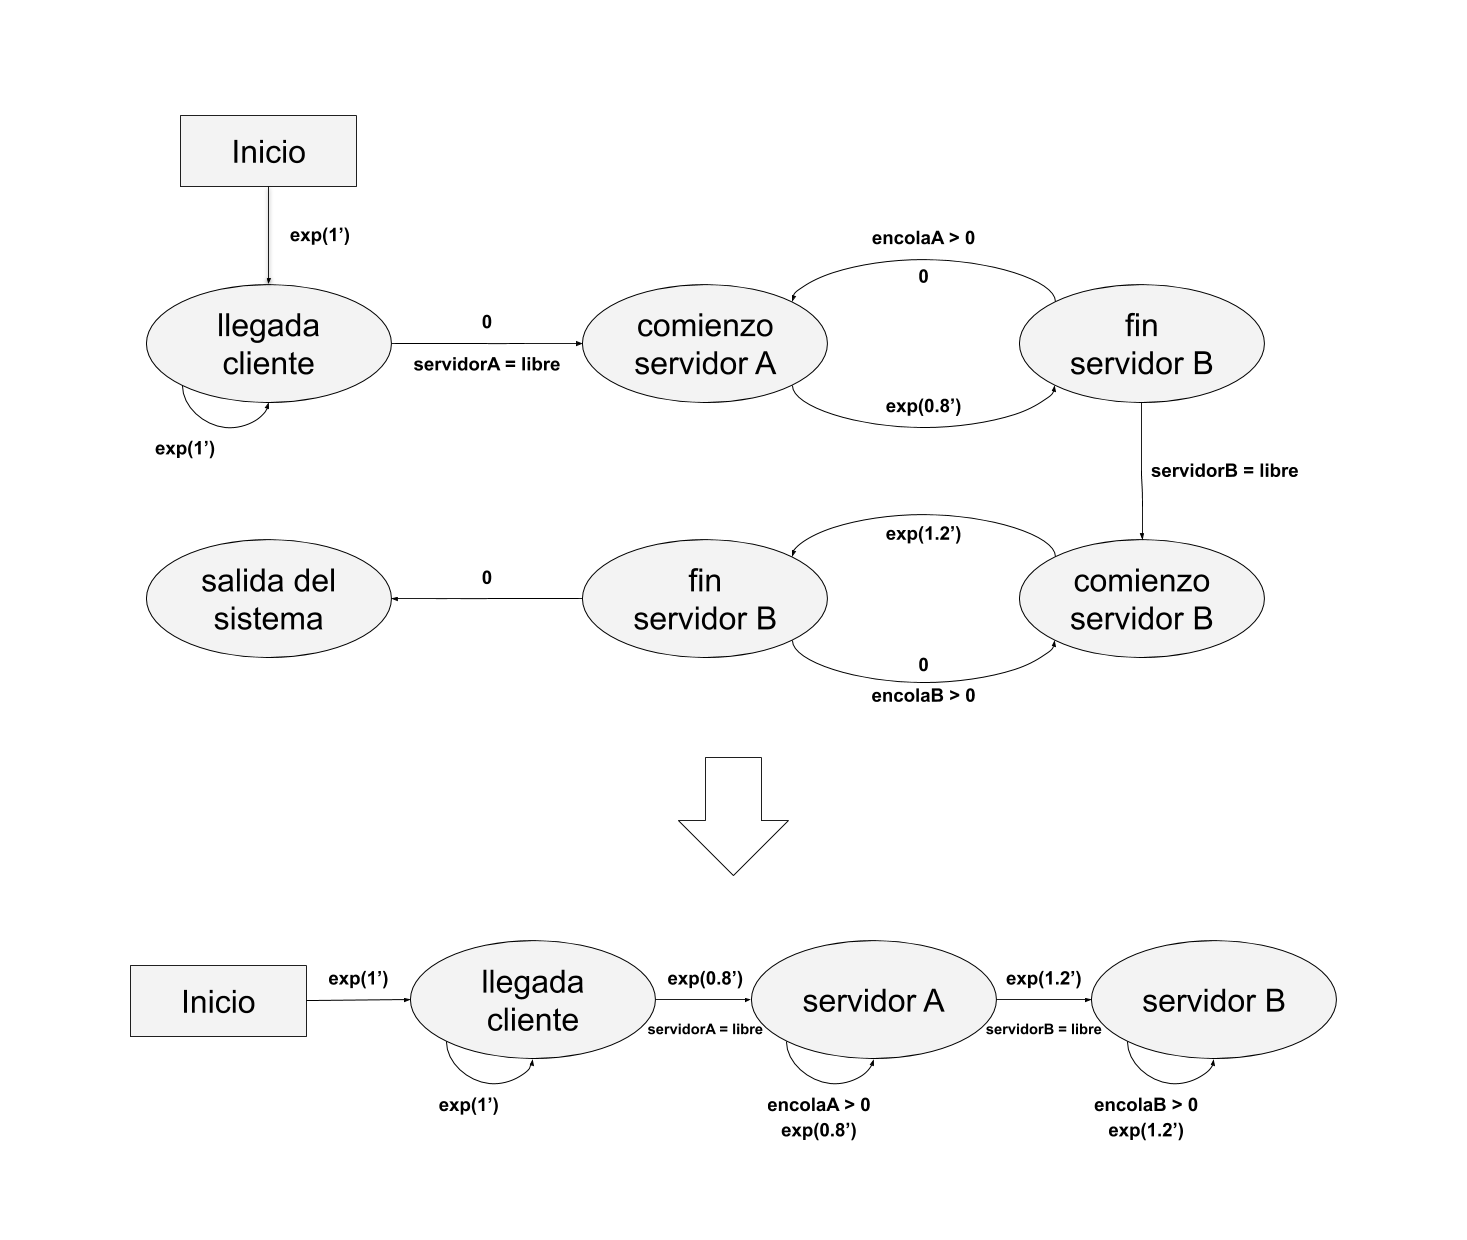
\includegraphics[scale=0.35]{img/grafo.png}
	\caption{Grafo de sucesos completo}
\end{figure}

\begin{figure}[H]
	\centering
	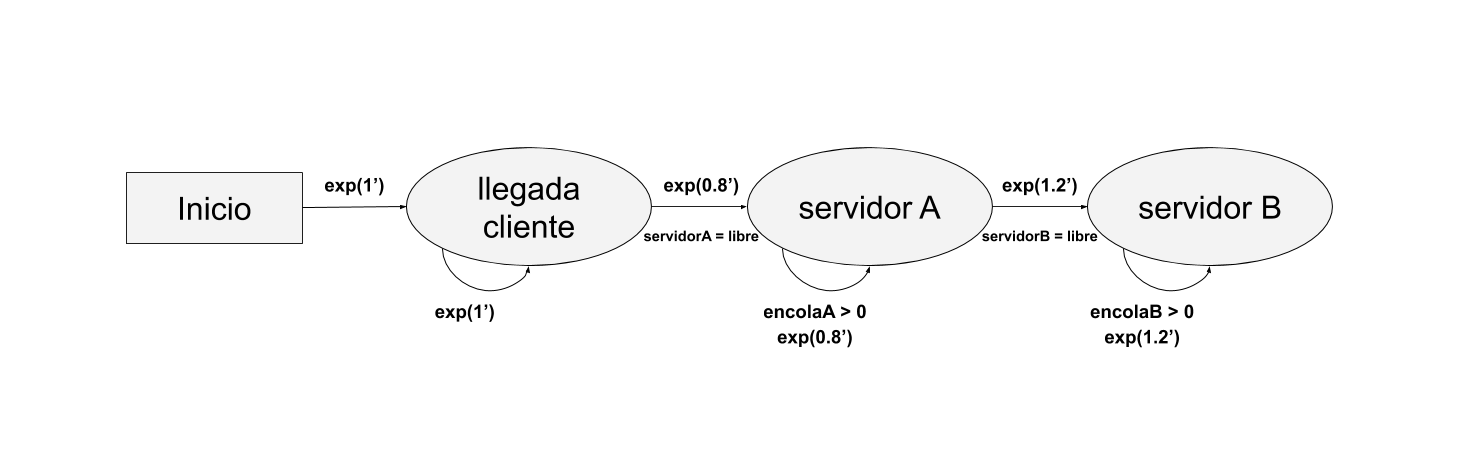
\includegraphics[scale=0.35]{img/grafo-reducido.png}
	\caption{Grafo de sucesos reducido}
\end{figure}

Ahora vamos a explicar cada uno de los sucesos detallando las rutinas, variables de inicialización y generador de informes. Lo primero que vamos a hacer será
mostrar la estructura ($struct$) de nuestra lista de sucesos. Como podremos observar insertaremos el suceso y el tiempo en el que se ha producido:
\begin{lstlisting}
	/* Estructura de la lista */
	typedef struct {
		int suceso;
		float tiempo;
	} suc;
	
\end{lstlisting}

También utilizaremos estas dos funciones para insertar elementos en la lista. Como será una lista ordenada por tiempo, la primera simplemente comparará uno con
otro, y la segunda, insertará dependiendo del valor obtenido en la función anterior:
\begin{lstlisting}

	/* Funcion de comparacion */
	bool compare(const suc &s1, const suc &s2)
	{ return s1.tiempo < s2.tiempo; }


	/* Inserta de forma ordenada un elemento en la lista de sucesos */
	void insertar_lsuc(suc n)
	{
	lsuc.push_back(n);

	// Mantener ordenada la lista por el tiempo de los sucesos
	lsuc.sort(compare);
	}
	
\end{lstlisting}

\newpage
Tras esto vamos a ver cómo se implementarán cada uno de los sucesos correspondientes a nuestro sistema:
\begin{lstlisting}
	/* Funcion del suceso llegada cliente */
	void llegada_cliente()
	{
		insertar(tiempos_llegadas, reloj);

		insertar(lsuc, llegada_cliente, sucActual, reloj+exp(1.0));

		if (servidorA == LIBRE){
			servidorA = OCUPADO;
			insertar(lsuc, llegada_servidorA, sucActual, reloj+exp(0.8));
		}
		else
			encolaA++;
	}
\end{lstlisting}

\begin{lstlisting}
	/* Funcion del suceso servidor A */
	void llegada_servidorA()
	{
		if (encolaA > 0){
			encolaA--;
			insertar(lsuc, llegada_servidorA, sucActual, reloj+exp(0.8));
		}
		else{
			servidorA = LIBRE;
		}

		if (servidorB == LIBRE){
			servidorB = OCUPADO;
			insertar(lsuc, llegada_servidorB, sucActual, reloj+exp(1.2));
		}
		else
			encolaB++;
	}
\end{lstlisting}

\begin{lstlisting}
	/* Funcion del suceso servidor B */
	void llegada_servidorB()
	{
		clientes_atendidos++;
		tiempo_clientes_sistema += reloj - tiempo_ultima_llegada;

		eliminar(tiempo_ultima_llegada);

		if (encolaB > 0){
			encolaB--;
			insertar(lsuc, llegada_servidorB, sucActual, reloj+exp(1.2));
		}
		else
			servidorB = LIBRE;
	}
\end{lstlisting}


Por último, vamos a mostrar la inicialización de las variables de interés y el generador de informes:
\begin{lstlisting}
	/* Inicializacion de las variables de interes */
	void inicializacion()
	{
		reloj = 0.0;
		tiempo_parada = 60.0 * 8;
		tiempo_clientes_sistema = 0.0;
		encolaA = 0;
		encolaB = 0;
		clientes_atendidos = 0;
		servidorA = LIBRE;
		servidorB = LIBRE;
	}

\end{lstlisting}

\begin{lstlisting}
	/* El generador de informes se encarga de calcular la media y
		 desviacion tipica de los valores obtenidos */
	void generador_informes(int simulaciones)
	{
		double media = sum / simulaciones,
				   desv = sqrt((sum2 - simulaciones * media * media) /
									(simulaciones - 1));

		// Mostrar resultados por pantalla
		printf("\n\nINFORME ->");
		printf("\nNumero de simulaciones: %d", simulaciones);
		printf("\nTiempo medio de estancia: %f \t desviacion: %f\n\n", media, desv);
	}
\end{lstlisting}


\section{Implementación del modelo}

En este apartado anterior ya hemos explicado cómo funcionan cada uno de los sucesos, pero no hemos comentado cómo se pone en marcha ni cómo utilizamos
el resto del modelo. Su funcionamiento es muy simnple. Lo primero que haremos será leer como parámetro del programa el número de simulaciones que vamos
a realizar. Posteriormente, pondremos en marcha un bucle con este número de simulaciones y el siguiente contenido:
\begin{lstlisting}

	for(int i = 0; i < simulaciones; i++)
	{
		// printf("\nSimulacion %d ...",cont_simu);
		inicializacion();
		while(parar==false)	{
			temporizacion();
			suceso();
		}
	}

\end{lstlisting}

Como podemos observar, para cada simulación inicializamos las variables (excepto los tiempos medios de estancia y desviación típica) y comenzamos con
la simulación del sistema. En ella ejecutamos las funciones de \textit{temporización()} y \textit{suceso()}, las cuales explicaremos a continuación.

\begin{lstlisting}
	/* Procedimiento temporizacion */
	void temporizacion()
	{
	sucActual = lsuc.front();
	lsuc.pop_front();
	reloj = sucActual.tiempo;
	}

\end{lstlisting}

Vemos que en esta función lo único que hacemos es actualizar el suceso actual al que esté primero en la lista, y también actualizamos el reloj con el
tiempo que tenga este último suceso seleccionado.

\begin{lstlisting}
	/* Procedimiento suceso */
	void suceso()
	{
	switch(sucActual.suceso)
		{
		case SUCESO_LLEGADA_CLIENTE: llegada_cliente(); break;
		case SUCESO_SERVIDOR_A: llegada_servidorA(); break;
		case SUCESO_SERVIDOR_B: llegada_servidorB(); break;
		case SUCESO_FIN_SIMULACION: fin_simulacion(); break;
		}
	}
	
\end{lstlisting}

En esta función elegimos el siguiente suceso a partir de lo obtenido en la función de \textit{temporizacion()}. Los sucesos que se pueden elegir son los
que definimos en el apartdo anterior, más el suceso \textit{fin-simulacion()} que simplemente para la ejecución del bucle y guarda los valores de las
sumatorias en sus variables correspondientes.


\newpage
\section{Experimentación y análisis del modelo}

Vamos a ejecutar nuestro modelo con un número alto de iteracciones, por ejemplo 1000, ya que su ejecución es bastante rápida. Cuantas más iteracciones
pongamos, más fiel a la realidad será nuestro modelo, teniendo siempre en cuenta la aleatoriedad del generador. Estos son los resultados que hemos
obtenido:

\begin{lstlisting}

	Tiempo clientes: 25572.724082 y clientes atendidos: 378
	Tiempo clientes: 8127.702767 y clientes atendidos: 410
	Tiempo clientes: 23624.744645 y clientes atendidos: 424
	Tiempo clientes: 17920.444762 y clientes atendidos: 377
	
	..................
	
	Tiempo clientes: 20845.240843 y clientes atendidos: 370
	Tiempo clientes: 26034.568622 y clientes atendidos: 409
	Tiempo clientes: 18660.893068 y clientes atendidos: 373
	Tiempo clientes: 33443.957111 y clientes atendidos: 361
	
	INFORME ->
	Numero de simulaciones: 1000
	Tiempo medio de estancia: 47.373443      desviacion: 14.080467
	
\end{lstlisting}
	
Como podemos ver, los tiempos medios en el servidor rondan los \textbf{47 segundos}. Puede parecer demasiado, ya que los tiempos que tardan en los
servicios son aleatorios exponenciales de 0.8 y 1.2 segundos; sin embargo, este valor tiene sentido, ya que en el servidor B se hace cuello de botella
al tardar un poco más que en el A. Esto hace que los clientes se acumulen en las colas y, por tanto, que el tiempo total del servidor aumente.

Ahora trataremos de reducir el tiempo medio de espera a 10 minutos, únicamente cambiando el tiempo del servidor B. Realizaremos varias ejecuciones con
distintos tiempos, bajando el exponencial a 1.2 y viendo cual es el valor límite en el que cambia. Este ha sido el resultado:

\begin{lstlisting}
	
	INFORME ->
	Tiempo en servidor B: exponencial 1.1		Numero de simulaciones: 1000
	Tiempo medio de estancia: 31.962392      desviacion: 12.615150

	INFORME ->
	Tiempo en servidor B: exponencial 1.0		Numero de simulaciones: 1000
	Tiempo medio de estancia: 19.010502      desviacion: 8.978181

	INFORME ->
	Tiempo en servidor B: exponencial 0.9		Numero de simulaciones: 1000
	Tiempo medio de estancia: 10.840208      desviacion: 4.544627

	INFORME ->
	Tiempo en servidor B: exponencial 0.85		Numero de simulaciones: 1000
	Tiempo medio de estancia: 8.949385       desviacion: 3.197139

\end{lstlisting}

Vemos que el valor del tiempo en el servidor B, debería ser una exponencial entre \textbf{0.9} y \textbf{0.85} minutos, aproximadamente, ya que también
tendremos en cuenta la aleatoriedad del sistema. Gracias a esto también podemos comprobar que en este servidor hay un cuello de botella, porque hemos
reducido el tiempo considerablemente bajando este valor, cosa que con el servidor A no nos ocurre (a continuación pondré una ejecución con el tiempo de
este reducido):

\begin{lstlisting}
	
	INFORME ->
	Tiempo en servidor A: exponencial 0.7		Numero de simulaciones: 1000
	Tiempo medio de estancia: 46.150444      desviacion: 14.835318
	
\end{lstlisting}


\end{document}

